\section{Distributed Deep Learning in Open Collaborations}
\label{sect:method}

There are two unsolved challenges that stand in the way of practical collaborative training. The first challenge is algorithmic: how to maintain optimal training performance with dynamically changing hardware and network conditions? Another major challenge is ensuring consistent training outcomes with inconsistent composition of participants. 
Thus, we organize this section around these two issues:

\begin{itemize}[leftmargin=*]
    \item Section~\ref{sect:method_general} provides a general overview of DeDLOC and explains how it maintains consistency in a dynamic environment.
    \item In Section~\ref{sect:method_algorithm}, we describe the generalized communication strategy that maximizes training throughput by adapting to the currently available devices.
    \item In Section~\ref{sect:method_system_design}, we address system design challenges, such as circumventing NAT and firewalls, training on large datasets and managing collaborator access.
\end{itemize}

\subsection{Ensuring training consistency}\label{sect:method_general}

Many state-of-the-art models, notably GANs~\cite{GAN} and Transformers~\cite{transformer}, require a strict training regimen. Deviating from the recommended batch size or introducing stale gradients may significantly affect the training outcome~\cite{trainingtips,liu-etal-2020-understanding,pipedream}. Since in a collaborative setting one has little control over the devices that participate in the experiment, it is almost guaranteed that the specific hardware setup will vary between runs and even during a single run. Without special precautions, these runs may result in models with vastly different final accuracy.

To avoid this pitfall, DeDLOC follows synchronous data-parallel training with fixed hyperparameters regardless of the number of collaborators. In order to compensate for relatively slow communication, we adopt training with extremely large batches~\cite{lars,lamb,trainingtips,kaplan2020scaling,gpt3}, which allows peers to communicate less frequently. This strategy also provides a natural way to deal with heterogeneous hardware~\cite{ott2018scaling}: each device accumulates gradients at its own pace until the collaboration reaches the target batch size. Once ready, the collaborators exchange their gradients and perform one optimizer step. Using synchronous updates makes DeDLOC mathematically equivalent to large-batch training on a regular HPC cluster; see Appendix~\ref{appendix:convergence_analysis} for a more detailed explanation. Figure~\ref{fig:collaborative_training} gives a high-level visual explanation of this algorithm.

\begin{figure}[b]
\vspace{-10pt}
    \centering
    % 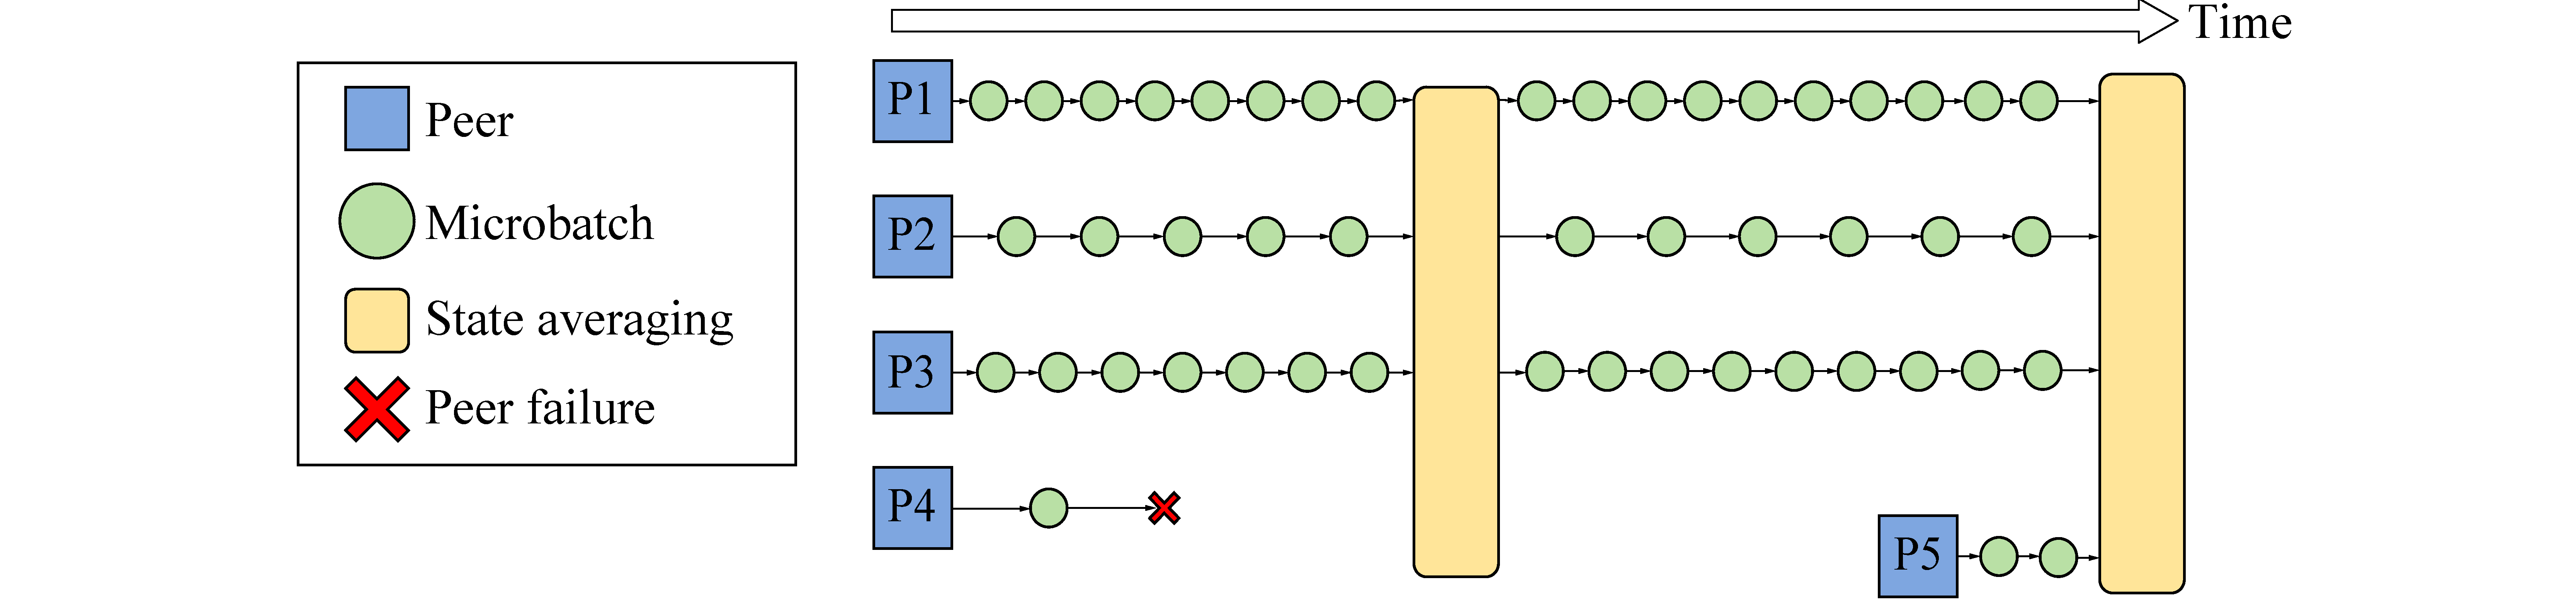
\includegraphics[height=160px]{resources/dedloc.pdf}
    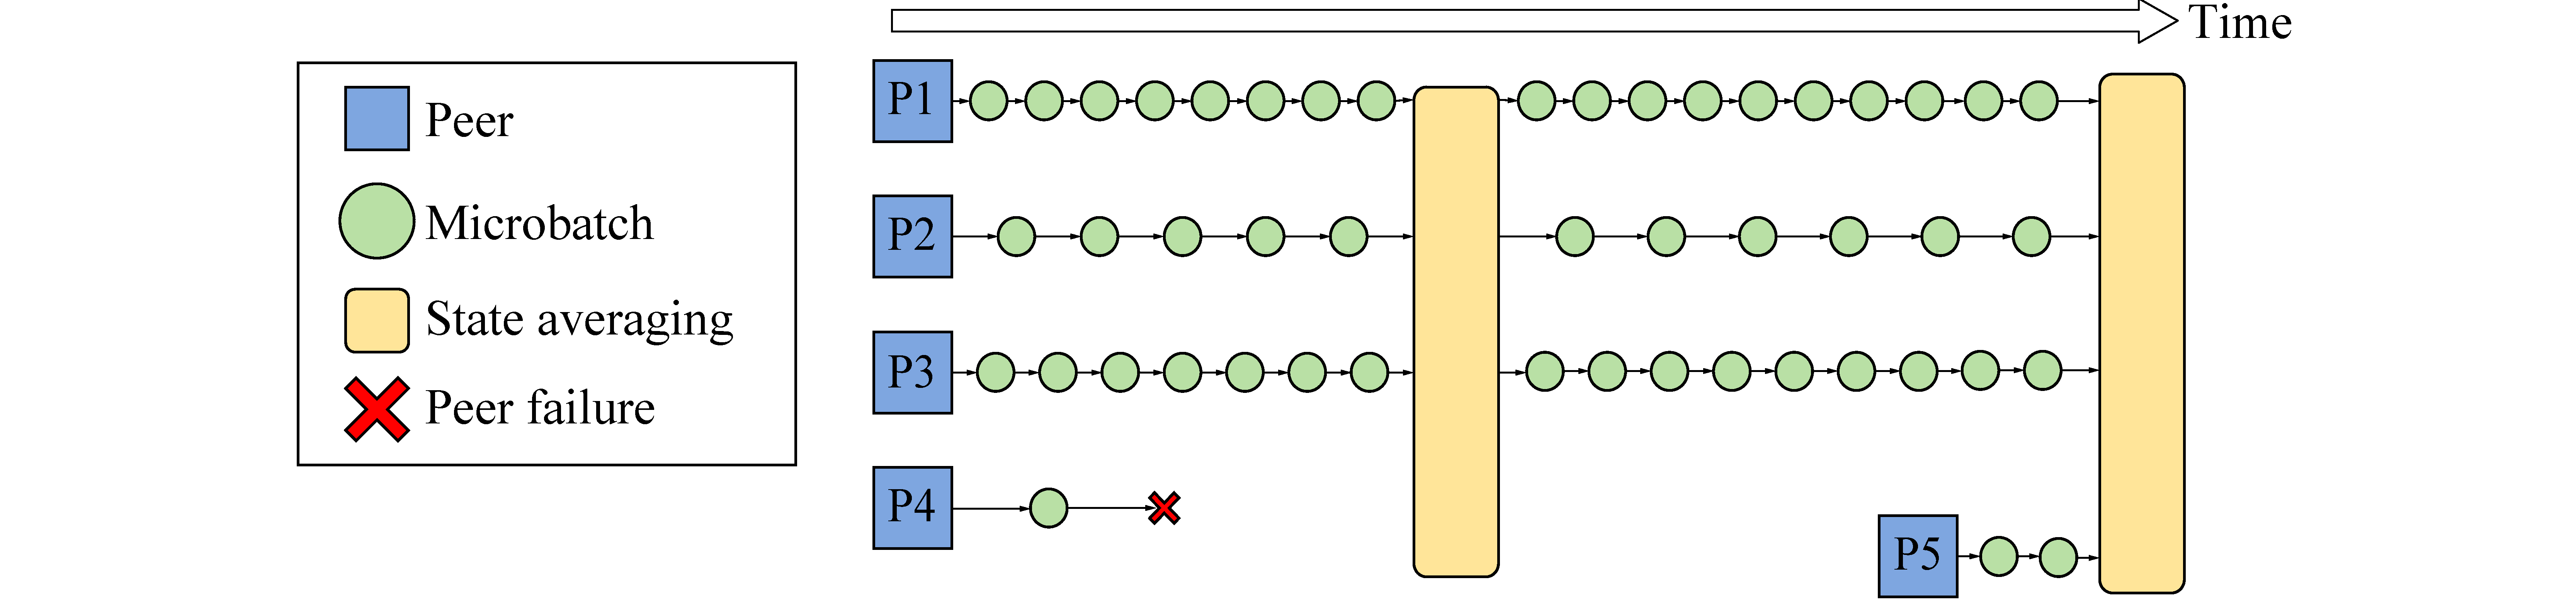
\includegraphics[height=100px]{resources/dedloc.pdf}
    \vspace{-8pt}
    \caption{Two DeDLOC training iterations with example collaborator dynamics.}
    \label{fig:collaborative_training}
    \vspace{-12px}
\end{figure}

\subsection{Adaptive averaging algorithm}\label{sect:method_algorithm}

As we discussed in Section~\ref{sect:related_distributed}, each distributed training algorithm has a narrow range of conditions where it can reach optimal performance. For instance, Ring All-Reduce works best on homogeneous hardware with low-latency communication, while Parameter Server strategy requires dedicated high-bandwidth devices that communicate with a large number of ``workers''. Since all devices are provided by volunteers, our training infrastructure is in a constant state of flux.

For instance, a collaboration can start with several homogeneous nodes that could be trained optimally with All-Reduce. If new participants bring devices with less bandwidth, it may be more efficient to use the original nodes as parameter servers. As more peers join, these servers will eventually become unable to handle the network load and the collaboration will need to switch to a different strategy.

Running efficient training on this kind of infrastructure requires a protocol that can dynamically assign roles to every peer given their hardware and network capabilities:
\begin{itemize}[leftmargin=*]
    \item \textbf{Compute performance:} Each peer $i \in 1,\ \dots,\ n$ can compute gradients over $s_i$ samples per second. A peer that is unable to compute gradients (i.e. that has no GPU) will have $s_i{=}0$.
    \item \textbf{Bandwidth:} Peers communicate with a limited throughput: $d_i$ for download and $u_i$ for upload.
    \item \textbf{Geographical limitations:} In addition to individual bandwidth, the communication throughput between two peers $i, j$ is also restricted by $t_{i j}$ and $t_{j i}$ in each direction.
\end{itemize}

Given these constraints, our objective is to find a communication strategy that has the highest training throughput, that is, the one that \textit{makes the most SGD steps with a target batch size $B$ per unit of time}. In turn, the training throughput of a collaboration depends on how we split the load among the participants. Each peer can be assigned to compute gradients over a subset of training examples, aggregate a part of those gradients from all peers, or both.

For simplicity and efficiency, we use delayed parameter updates (DPU)~\cite{zerooffload} --- a technique that allows gradient computation and communication to run in parallel, at the cost of exactly one round of staleness. This strategy can improve time to convergence for a wide range of models, including Transformers~\cite{zerooffload,aji2019making}. That said, our approach can be easily adapted to non-concurrent updates.

With DPU, the frequency of training updates is determined by either the time to compute gradients or the time to aggregate them, whichever takes longer. In total, a collaboration processes $\sum_{i=1}^{n} s_i \cdot c_i$ samples per second, where $c_i$ is the binary indicator denoting whether $i$-th peer is assigned to contribute gradients. Assuming the target batch size $B$, the frequency of the computation phase can be expressed as $F_{compute} = \sum_{i=1}^{n} s_i \cdot c_i \text{  } / \space B$.

During the communication phase, each peer is first assigned to accumulate gradients over a fraction of model parameters. After that, everyone partitions their local gradients and sends each partition to the corresponding peer. On the other end, receiver nodes accumulate the gradients from all senders and return the average. In modern distributed training systems, this procedure is highly parallelized~\cite{byteps,pytorch_distributed}: a reducer can aggregate one chunk of gradients while downloading the next chunk and distributing the previous one back to the same senders.

In order to properly optimize the training throughput, we must account for this parallelism. As such, we explicitly define the speed $a_{i j}$ at which peer $i$ sends gradients to peer $j$ for aggregation. In turn, $j$-th peer aggregates gradients from all peers at the rate of the slowest sender $a_j = \min_{i : c_i = 1} a_{i j}$. The senders can then get the aggregated results from the $j$-th reducer at $g_{j i} \leq a_j$. Finally, the total $a_{i j}$ and $g_{i j}$ for each peer cannot exceed their maximum download/upload speed. The only exception is that transfer within one node ($a_{i i}, \ g_{i i}$) does not count towards network throughput.

The frequency of the gradient aggregation phase is simply the rate at which the slowest peer can aggregate the full gradient vector: $F_{agg} = \min_i {\sum_{j} g_{j i}} \text{ } / \text{ }P$ , where $P$ is the number of model parameters. The final optimization problem can be formulated as follows:
% TODO (mryab) \include{optidef}
\begin{equation}
\label{eq:main_problem}
\begin{array}{rclll}
\underset{a, g, c}{\max} & &
                                \min\Bigg(\frac{\sum_{i=1}^n s_i \cdot c_i }{B},\ 
                                     \frac{ \min_i\sum_{j} g_{j i}}{P}\Bigg)&\quad&\\
\textrm{s.t. } &\quad & g_{i j} \leq \min_{k: c_k{=}1} a_{k i}  &\quad&\forall i, j \\
                 & \quad  & \sum_{j \neq i}\left( a_{j i} + g_{j i}\right) \leq d_{i} & \quad&\forall i \\
                 & \quad &   \sum_{j \neq i}\left( a_{i j} + g_{i j}\right) \leq u_{i} & \quad&\forall i \\
                 & \quad &   a_{i j} + g_{i j} \leq t_{i j} & \quad&\forall i, j \\
\end{array}
\end{equation}


This problem must be solved regularly as participants are joining and leaving. Thus, we must ensure that the benefits of the optimal strategy outweigh the overhead of computing it. For that reason, we formulate optimal strategy search as a linear program that can be solved efficiently\footnote{In our experiments, the LP solver consistently converged in  $<$ 50ms and was called $\approx$ 2 times per minute.}. A more formal definition of problem~\eqref{eq:main_problem} with detailed LP reduction can be found in Appendix~\ref{appendix:lp_optimization}.

After this problem is solved, we assign each peer to aggregate a fraction of gradients proportional to $\min_j g_{ji}$. Peers with $c_i{=}1$ are also tasked with computing the gradients, while peers with $c_i{=}0$ remain idle and only participate in communication. This results in a natural division of labor. In the presence of many compute-heavy peers, some participants without accelerators will dedicate all their bandwidth to gradient aggregation instead of sending their local gradients.

\textbf{Node failures.} The resulting procedure can find the optimal communication strategy for averaging gradients across all participants. However, as the number of participants grows, it might be impractical to compute the global average due to node failures. Based on our experiments with several hundred active volunteers, most training iterations will have at least one participant with network issues. This implies that without necessary precautions, the entire averaging round will fail more often than it will succeed. %This implies that the averaging protocol will fail more often than it will succeed.
To combat this issue, we use techniques~\cite{moshpit,wagma} that replace global averaging with several consecutive iterations in alternating groups of size $m$. The groups are chosen in such a way that the collaboration can obtain the exact average in $\log_m n$ steps. Furthermore, if any single participant fails, it will only affect his immediate group rather than the entire collaboration.

We adaptively choose the optimal group size $m$ based on the number of peers and their failure rates. This optimization problem is independent of Equation~\eqref{eq:main_problem} and aims to maximize the rate at which collaborators can compute the global average. We elaborate on this procedure in Appendix~\ref{appendix:groups}.

\textbf{Comparison with existing techniques.} Our method was designed as a generalization of existing data-parallel strategies that recovers them in special cases. To illustrate this idea, we provide example configurations for which DeDLOC recovers specific well-known strategies:

\begin{enumerate}[leftmargin=*]
    \item \textbf{AR-SGD:} a homogeneous collaboration with reliable peers will use Butterfly All-Reduce~\cite{butterfly_arsgd};
    \item \textbf{Parameter Server:} adding a single participant with a very high bandwidth and low compute performance will turn the previous collaboration into a parameter server~\cite{ps};
    \item \textbf{BytePS:} participants with the same bandwidth as AR-SGD nodes, but without compute accelerators, will behave as auxiliary summation services from BytePS~\cite{byteps};
    \item \textbf{Decentralized SGD:} any collaboration with a sufficiently high failure rate will converge to $m{=}2$. In this mode, all communication is performed between pairs of nodes, similarly to D-PSGD~\cite{dp_sgd}.
\end{enumerate}

However, when training with actual volunteer devices, DeDLOC typically follows a hybrid communication scheme that differs from each of the above options. We display several examples of schemes that can arise as a solution for the optimal strategy search problem in Figure~\ref{fig:examples}.

\begin{figure}[t]
    \centering
    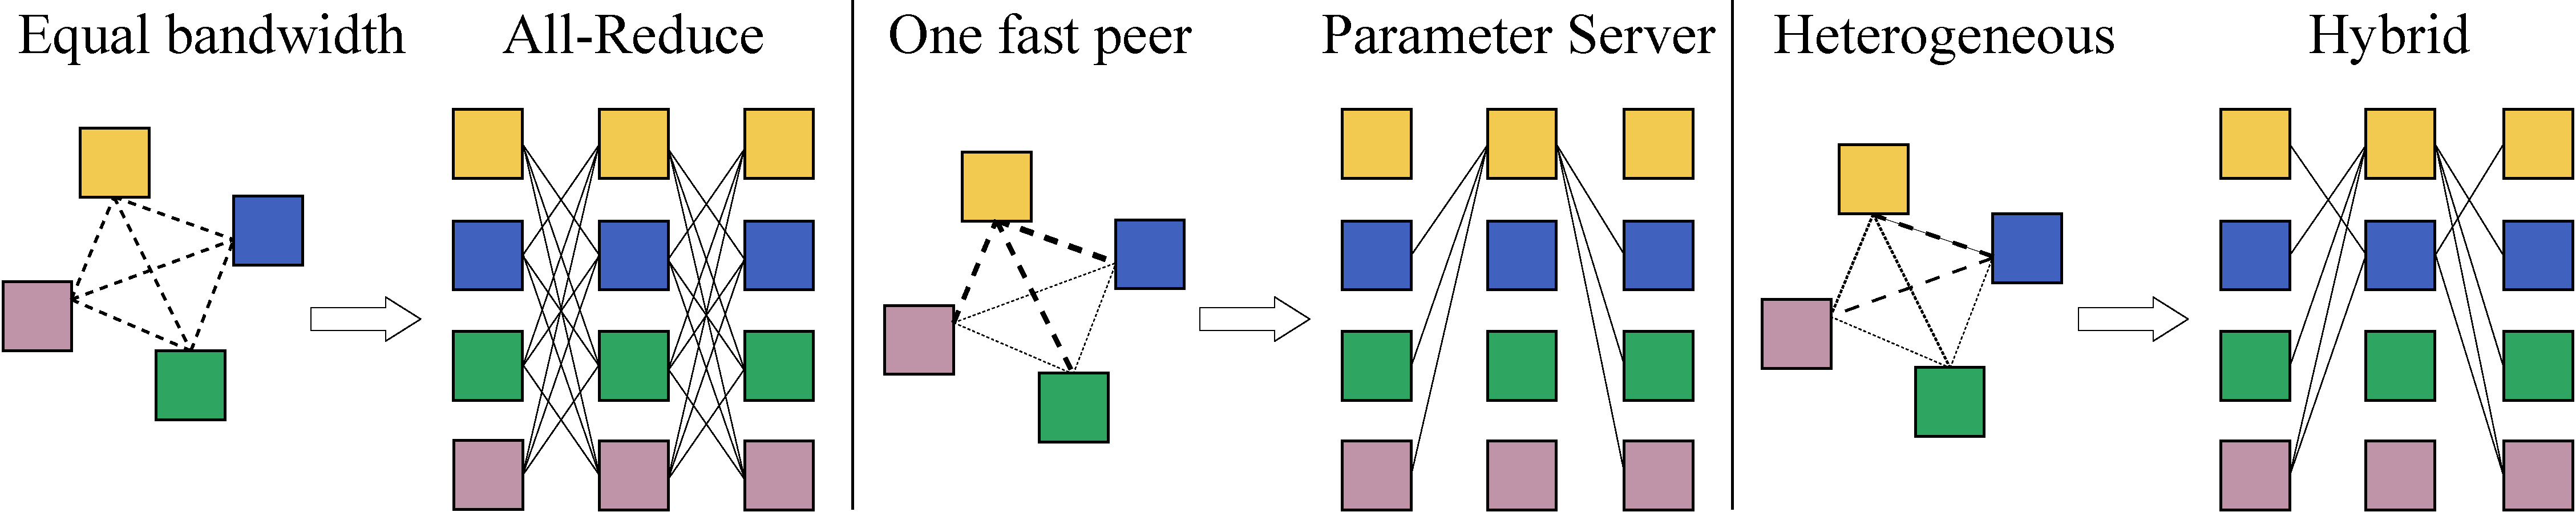
\includegraphics[height=78px]{resources/adaptive.pdf}
    \caption{Example collaboration setups and corresponding strategies for optimal averaging. Each square represents one of the peers, line thickness denotes pairwise connection speed.}
    \label{fig:examples}
    \vspace{-12pt}
\end{figure}

\vspace{-2pt}
\subsection{System design}\label{sect:method_system_design}

Training with volunteer hardware requires specialized system architecture that can dynamically scale with collaboration size and recover from node failures. DeDLOC achieves these properties by operating as a swarm, similarly in spirit to BitTorrent~\cite{torrent} and I2P~\cite{i2p}. Individual peers coordinate by forming a Distributed Hash Table --- a fully decentralized fault-tolerant key-value storage~\cite{kademlia,kaashoek2003koorde}. Collaborators use this shared ``dictionary'' to count the number of accumulated gradients, find groups for averaging and keep track of the training progress.

DeDLOC ensures that all peers use up-to-date parameters by tracking the number of global steps of each peer. If a peer skips a step, it will observe that others made more steps and download the latest parameters and optimizer statistics from one of the up-to-date peers before resuming training. 
% Similarly, if a peer joins during the experiment, it will download the state from an up-to-date peer.

In order to ensure the integrity of DHT throughout the training run, DeDLOC requires a few peers with stable internet access. These ``backbone'' peers are responsible for welcoming new collaborators and performing auxiliary functions, such as storing checkpoints and tracking learning curves. The only requirement for those peers is that at least one of them is available at all times. As such, the backbone peers can be hosted on inexpensive servers without GPU (see Appendix~\ref{appendix:cost_analysis} for cost analysis).

All other devices are treated as regular collaborators. Depending on their hardware and network bandwidth, these devices can be assigned to (i) compute gradients, (ii) aggregate gradients computed by other peers or (iii) do both, according to the adaptive averaging algorithm. However, performing these steps with actual volunteer devices requires solving another set of challenges described below.

\vspace{-4pt}
\paragraph{Training under NAT and firewalls.}In addition to having uneven compute and network capabilities, volunteer devices also deviate from traditional servers in network configuration. One major difference is the use of Network Address Translation (NAT)~\cite{Biggadike05natblaster:establishing} --- the technology that allows multiple devices to share the same IP address. In practice, the majority of household and organizational computers around the world use one or multiple layers of NAT (see Appendix~\ref{appendix:nat_firewall} for more details). Unfortunately for distributed training, NAT makes it harder to establish peer-to-peer connections~\cite{hole_punching}.

When operating under NAT, DeDLOC participants use one of the following techniques:

\vspace{-4pt}
\begin{enumerate}[leftmargin=*]
    \item \textbf{Hole punching:} use a third peer to temporarily open access to both devices. Once both peers are accessible, they can establish a direct connection and transfer data as usual~\cite{hole_punching};
    \item \textbf{Circuit relays:} both devices connect to a relay (another peer that is mutually accessible), then forward all communication through that relay~\cite{TURN};
    \item \textbf{Client mode:} if everything else fails, a peer can still send gradients to others without the need for incoming connections. This imposes an additional constraint $a_i=0$ for Equation~\eqref{eq:main_problem}.
\end{enumerate}
\vspace{-4pt}

A similar set of strategies can be found in a wide range of distributed systems that rely on peer-to-peer communication, such as WebRTC, VoIP (IP telephony), and BitTorrent. Most of these systems rely on dedicated servers to establish connections between peers. However, in our case it is more appealing to use a fully decentralized NAT traversal where the regular peers perform hole punching and relaying by themselves. We describe this approach in more detail in Appendix~\ref{appendix:p2p}.

\vspace{-4pt}
\paragraph{Training on large datasets.} Many prospective applications of DeDLOC require training on large datasets that can take multiple hours to download. We circumvent this problem by allowing participants to download the data progressively during training. To support this behavior, we split the dataset into shards; upon joining the collaboration, a peer begins downloading examples shard by shard in a streaming fashion. Once the first several examples are obtained, a collaborator can begin training right away while downloading the rest of data in background.

To ensure that the training examples are independent and identically distributed, each participant loads shards in a different random order and uses a buffer to shuffle the data within each shard. Each participant loads the first $S=10,000$ examples into a buffer, then randomly picks a training batch from this buffer and replaces the chosen examples with newly downloaded ones. In our experiments, we stream the training data from a dedicated storage service. However, this service can be replaced with a peer-to-peer data sharing protocol akin to BitTorrent; see Appendix~\ref{appendix:decentralized_dataset_streaming} for details.


% The examples are loaded chunk by chunk from remote files in a streaming fashion. To ensure that we get shuffled datasets, we first make sure that each participant shuffles the dataset shards order. We also use a shuffle buffer: each participant loads the first 10,000 examples into a buffer, then the data loader randomly picks examples from this buffer, and the chosen examples are replaced with new ones in the buffer.

% This allows each participant to start training directly instead of waiting for all the data to be downloaded to their device. 
% Moreover, since the tokenization and masking are done on-the-fly by the participants during training, no data preprocessing is needed before starting the experiment.

% The examples are loaded chunk by chunk from remote files in a streaming fashion. To ensure that we get shuffled datasets, we first make sure that each participant shuffles the dataset shards order. We also use a shuffle buffer: each participant loads the first 10,000 examples into a buffer, then the data loader randomly picks examples from this buffer, and the chosen examples are replaced with new ones in the buffer.

\vspace{-4pt}
\paragraph{Collaborator authentication.} Many prospective applications of DeDLOC need a way to keep track of individual peer contributions and protect against malicious peers. In our experiments, we achieve this using an allowlist authentication system that we describe in Appendix~\ref{appendix:authorization}.


%                                  \\\\\       \\\\\
%      \\\\__.  \\\\__.  \\\\__.  \\\\\\\__.  \\\\\\\__o
% _____\\\\'/___\\\\'/___\\\\'/___\\\\\\\'/___\\\\\\\'/____
% This paper is infested with hedgehogs. Run for your life!